% !TeX spellcheck = it
\chapter*{Introduzione}
\markboth{Introduzione}{Introduzione}
\addcontentsline{toc}{chapter}{Introduzione}
\thispagestyle{empty}
--Aggiungere in testa motivazioni del lavoro, stato dell’arte della geolocalizzazione indoor e quali problemi si vogliono risolvere--
\newline\newline
Il lavoro di questa tesi si colloca nel progetto aziendale Tekne per la realizzazione di un sistema di geolocalizzazione di operatori in contesti privi di segnale GPS.
Il sistema permette ad un “esploratore” di creare dinamicamente una rete di nodi all’interno di zone nelle quali il segnale GPS è assente o comunque debole. Questa rete verrà poi ampliata ed utilizzata dagli operatori successivi ad esso per geolocalizzarsi all’interno della zona ed intervenire in maniera ottimale. \\
Uno scenario esemplificativo è quello di un vigile del fuoco che interviene in un edificio per soccorrere una persona. Tale operatore è considerato un esploratore, poiché è il primo ad intervenire e la planimetria dell’edificio risulta essere ignota e/o cambiata a seguito dell’evento disastroso (Fig.\ref{fig:planOriginale} e Fig.\ref{fig:planAlterata}). 

\begin{figure}[h]
	\begin{minipage}[b]{6cm}
		\centering
		\includegraphics[scale=0.35]{Introduzione/piantina1.png}
		\caption{Planimetria originale}
		\label{fig:planOriginale}
	\end{minipage}
	\ \hspace{10 mm} \
	\begin{minipage}[b]{6cm}
		\centering
		\includegraphics[scale=0.35]{Introduzione/piantina2.png}
		\caption{Planimetria alterata}
		\label{fig:planAlterata}
	\end{minipage}
\end{figure}

\newpage
I rettangoli in grigio (Fig.\ref{fig:planAlterata}) rappresentano aree non più accessibili dell’edificio, mentre le mura interrotte nuovi percorsi creati a causa dei crolli. 
Durante tutta la fase di scouting, l’esploratore posizionerà un’ancora (nodo) ogni qualvolta il raggio della precedente risulti essere al limite. Così facendo si “lascerà dietro una scia di briciole” che gli permetteranno di orientarsi all’interno dell’edificio, di eseguire il percorso all’inverso o di ricevere supporto da un’ulteriore operatore. Nelle figure seguenti, si può notare come la rete cresca man mano che l'esploratore avanza all'interno dell'edificio.

\begin{figure}[h]
	\begin{minipage}[b]{6cm}
		\centering
		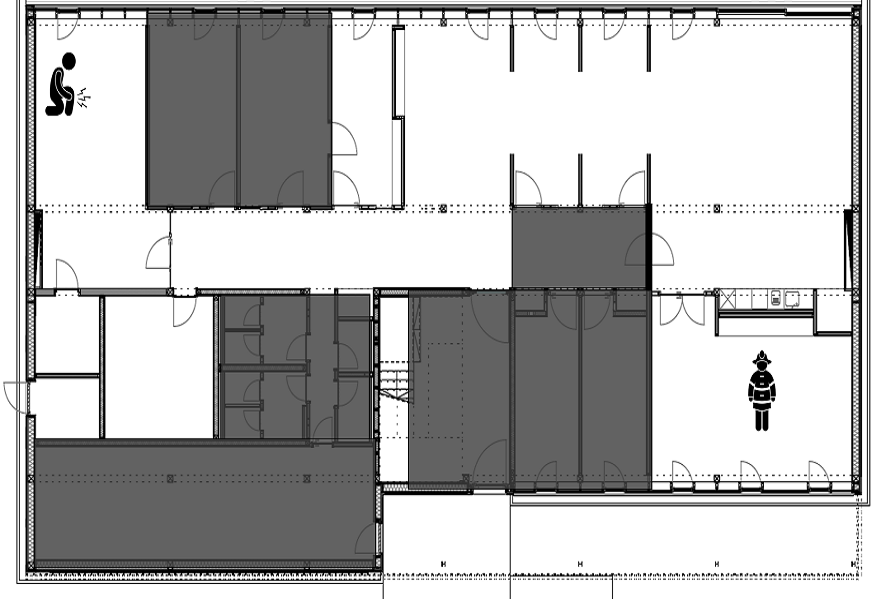
\includegraphics[scale=0.35]{Introduzione/intervento_step_0.png}
		\caption{Rete allo step 0 dell'esploratore}
		\label{fig:step0}
	\end{minipage}
	\ \hspace{10 mm} \
	\begin{minipage}[b]{6cm}
		\centering
		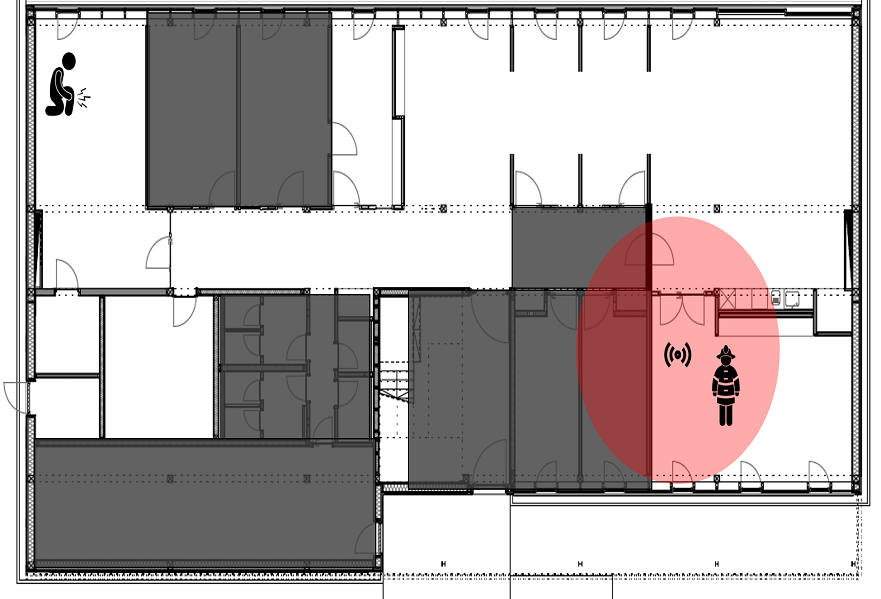
\includegraphics[scale=0.35]{Introduzione/intervento_step_1.png}
		\caption{Rete allo step 1 dell'esploratore}
		\label{fig:step1}
	\end{minipage}
\end{figure}


\begin{figure}[h]
	\begin{minipage}[b]{6cm}
		\centering
		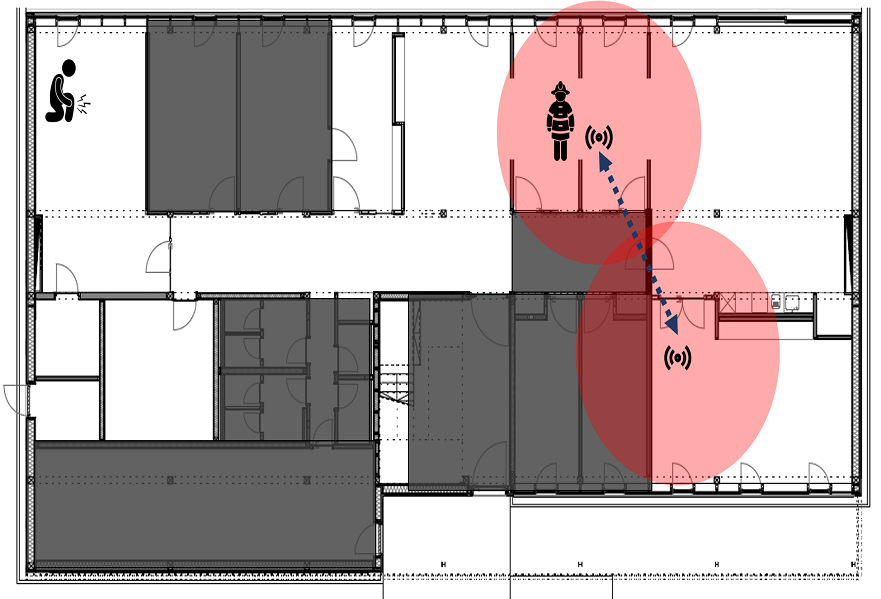
\includegraphics[scale=0.35]{Introduzione/intervento_step_2.png}
		\caption{Rete allo step 2 dell'esploratore}
		\label{fig:step2}
	\end{minipage}
	\ \hspace{10 mm} \
	\begin{minipage}[b]{6cm}
		\centering
		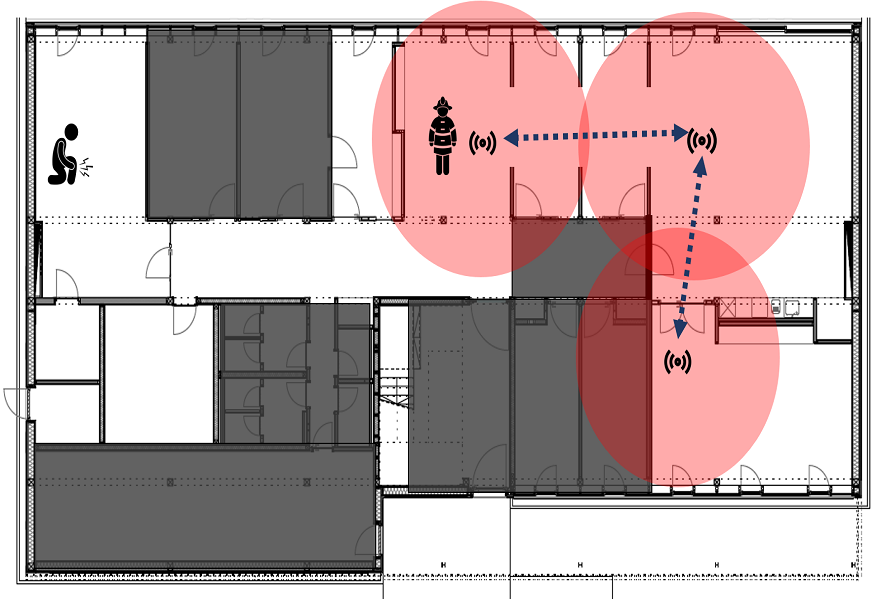
\includegraphics[scale=0.35]{Introduzione/intervento_step_3.png}
		\caption{Rete allo step 3 dell'esploratore}
		\label{fig:step3}
	\end{minipage}
\end{figure}

\begin{figure}[h]
	\begin{minipage}[b]{6cm}
		\centering
		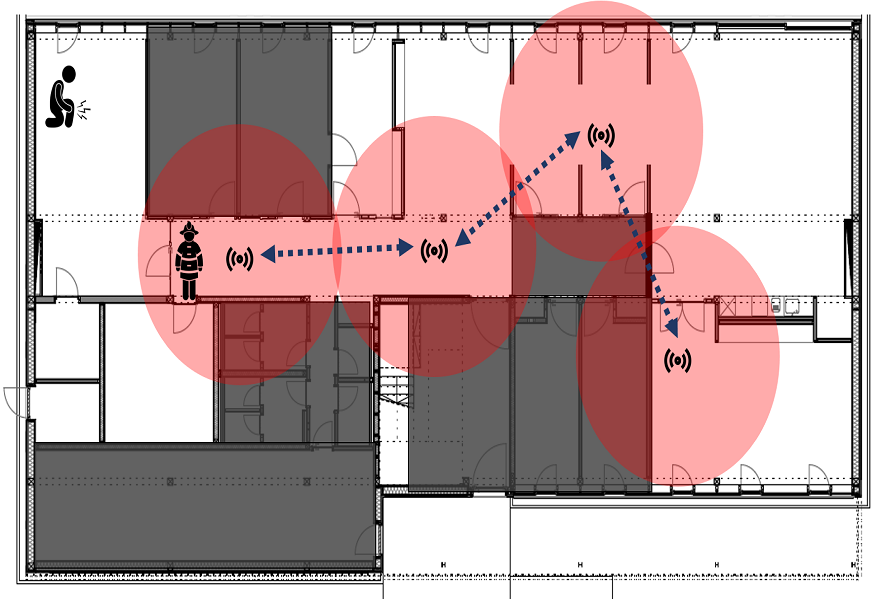
\includegraphics[scale=0.35]{Introduzione/intervento_step_4.png}
		\caption{Rete allo step 4 dell'esploratore}
		\label{fig:step4}
	\end{minipage}
	\ \hspace{10 mm} \
	\begin{minipage}[b]{6cm}
		\centering
		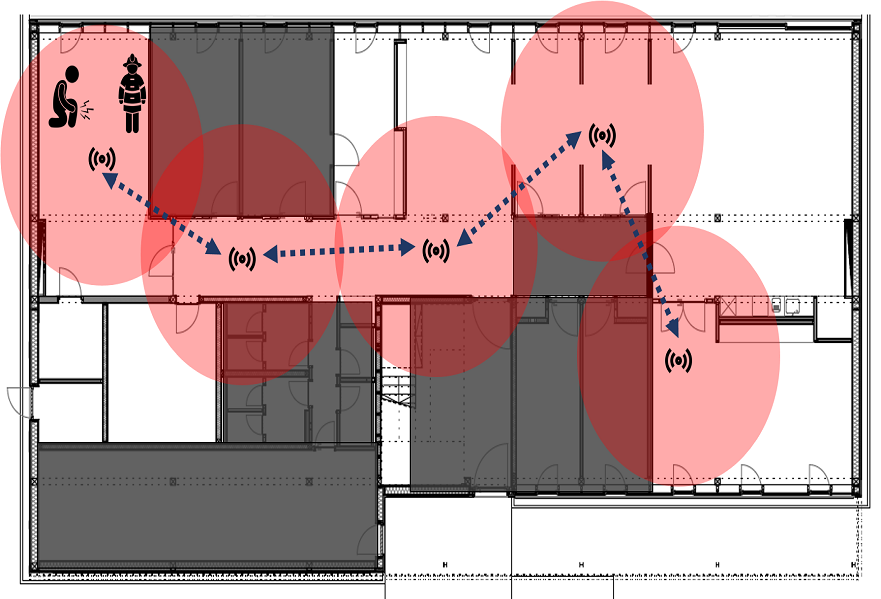
\includegraphics[scale=0.35]{Introduzione/intervento_step_5.png}
		\caption{Rete allo step 5 dell'esploratore}
		\label{fig:step5}
	\end{minipage}
\end{figure}
\newpage
Una volta creata l’infrastruttura, gli operatori potranno comunicare e condividere informazioni come posizione e stato. \newline
La presente tesi è così strutturata:
\begin{description}
\item [Capitolo 1:] Viene descrito il sistema e le parti realizzate nel contesto di questa tesi.
\item [Capitolo 2:] Vengono illustrate le tecnologie utilizzate (sensori MEMS e UWB).
\item [Capitolo 3:] Viene descritto il rumore dei dati grezzi, le tecniche di raffinamento e alcuni algoritmi per la fusione dei dati.
\item [Capitolo 4:] Si riporta l'implementazione software e hardware del sottosistema.
\item [Capitolo 5:] Viene illustrato il procedimento di validazione e l'analisi dei dati ottenuti mediante algoritmi di data fusion.
\end{description}